\documentclass[../Hovedrapport.tex]{subfiles}
\newcommand{\gray}{\rowcolor[gray]{0.95}}
\begin{document}
%\vspace{-30pt}
%------------------------------------------------------------------------------
\section{Kontrol af kondensatorydelse (J.K. \& C.R.)}
    \label{sec:dim_kondensator}
I det følgende afsnit vil kondensatorydelsen blive beregnet for en udvalgt varmeveksler. Den er via en iterativ proces blevet beregnet til at være af samme type som varmesksleren, der bruges som fordamper. Sidstnævnte er beregnet i afsnit \ref{sec:dim_fordamper}.

\subsection{Antagelser  (J.K. \& C.R.)}
Kondensatorydelsen beregnes ud fra varmeovergangstallene udvendigt og indvendigt, samt de tre termiske modstande vist på figur \ref{fig:modstande_i_roer}. Disse benyttes til at beregne en kondensatorkapacitet, der sammenholdes med den kapacitet, som kompressoren kan sikre ved dens maksimale omdrejningstal. Kondensatoren vil blive betragtet som en ribberørsvarmeveksler, hvorfor samme fremgangsmåde benyttes som ved beregning af fordamperen i afsnit \ref{sec:dim_fordamper}.

Som tidligere nævnt vil beregningerne blive foretaget efter en kondenseringtemperatur på \SI{50}{\celsius} jf. afsnit \ref{sec:noegletal}
Der gættes på en udblæsningstemperatur på \SI{35}{\celsius}, som vil blive præciseret via en iterativ proces. Denne beregningsproces består af tilpasning af udblæsningstemperaturen, således at denne er sammenfaldende med en teoretisk udblæsningstemperatur beregnet ud fra kondensatorydelsen. 

Ved en kondenseringstemperatur på $\SI{50}{\celsius}$ og fordampningstemperatur på $\SI{-8}{\celsius}$ samt et omdrejningstal for kompressoren på $\SI{4000}{RPM}$ skal kondensatoren have en kondenseringsydelse på $\SI{530}{\watt}$, hvilket kondensatoren dimensioneres efter jf. \citep{Coolselector}. Denne kondenseringsydelse er forskellig fra den fundet i afsnit \ref{sec:kondenseringsydelse_med_koling}, hvilket skyldes at \textit{Coolselector} ikke tager højde for køling af kompressoren.

Kondensatoren har, som tidligere nævnt, samme dimensioner som fordamperen, og de fysiske størrelser samt dimensioner fremgår af figur \ref{fig:varmevekslerdim1} og \ref{fig:varmevekslerdim2} under afsnit \ref{sec:dim_fordamper}. I nedenstående tabel \ref{tab:Kondensator_anlægs_Data} fremgår det, hvilke antagelser og data, der er brugt i beregningen af kondensatorydelsen.
%------------------------------Tabel med dimensioner af anlægget, kommenteret ud---------------------------
%\begin{table}[H] 
%	\centering
	% \caption*{\textbf{\large Kondensatordata}} 
	% \vspace{-0.3cm}
%	\begin{tabular}{|c|l|l|c|}  \rowcolor[gray]{0.5}                                \hline
%	\multicolumn{4}{|c|}{\textbf{Kondensatordata}}                               \\ \hline \rowcolor[gray]{.8}
%	\textbf{Variabel}   & \textbf{Værdi}        & \textbf{Forklaring}       & \textbf{Kilde}    \\ \hline \rowcolor[gray]{.95}
%	L_\text{rør}        & \SI{5,28}{\meter}     & Rørlængde i kondensator   & Målt              \\ \hline \rowcolor[gray]{.95} 
%	d_\text{i}          & \SI{7}{\milli\meter}  & Indre rørdiameter         & Målt              \\ \hline \rowcolor[gray]{.95}
%	d_\text{y}          & \SI{8}{\milli\meter}  & Ydre rørdiameter          & Målt              \\ \hline \rowcolor[gray]{.95}
%	b_\text{ribber}     & \SI{0,037}{\meter}    & Ribbebredde               & Målt              \\ \hline \rowcolor[gray]{.95}
%	h_\text{ribber}     & \SI{0,2}{\meter}      & Ribbehøjde                & Målt              \\ \hline \rowcolor[gray]{.95}
%	t_\text{ribber}     & \SI{0,001}{\meter}    & Ribbetykkelse             & Målt              \\ \hline \rowcolor[gray]{.95}
%	N_\text{ribber}     & 71                    & Antallet af ribber        & Målt              \\ \hline \rowcolor[gray]{.95}
%	N_\text{rørrækker}  & 3                     & Antallet af rørrækker     & Målt              \\ \hline \rowcolor[gray]{.95}
%	N_\text{rør}        & 24                    & Antallet af rør           & Målt              \\ \hline \rowcolor[gray]{.95}
%	N_\text{serie}      & 1                     & Antal kondensatore i serie& Målt              \\ \hline \rowcolor[gray]{.5}
%	\end{tabular} 
%	\caption{\textit{Variabeloversigt til dimensionering af kondensatoren}} 
%	\label{tab:kondensator_Data} 
%	\vspace{-20pt}
%\end{table} \\ \\

\begin{table}[H] 
	\centering
%	    \caption*{\textbf{\large Fordamper data}} 
%	    \vspace{-0.3cm}
	\begin{tabular}{|c|c|c|c|}  \rowcolor[gray]{0.7}                                \hline
	\multicolumn{4}{|c|}{\textbf{Variabler til beregning af kondensatorydelse}}                                                   \\ \hline \rowcolor[gray]{.8}
	\textbf{Variabel}   & \textbf{Værdi}        & \textbf{Forklaring}       & \textbf{Kilde}    \\ \hline  
	x_\text{g}          & 1                     & Dampkvalitet - mættet gas   &  \\ \hline 
	x_\text{l}          & 0                     & Dampkvalitet - mættet væske &  \\ \hline 
%	g                   & \SI{9,82}{m/s^2}      & Tyngdeaccelerationen                        & \\ \hline \rowcolor[gray]{.95}
%	C                   & 0,41                  & Faktor C for fortsatte røranordning         & Aages noter \\ \hline \rowcolor[gray]{.95}   
%	m                   & 0,60                  & Eksponent m for fortsatte røranordning      & Aages noter \\ \hline \rowcolor[gray]{.95}
	t_\text{k}          & \SI{50}{\celsius}     & Kondenseringstemperaturen                   & Antagelse  \\ \hline 
	t_\text{c}        & \SI{30}{\celsius}     & Lufttemperaturen før kondensatoren          & Figur \ref{fig:Konden_tempforloeb_antaget}   \\ \hline 
	t_\text{d}        & \SI{35}{\celsius}  & Lufttemperaturen efter kondensatoren        & Figur \ref{fig:Konden_tempforloeb_antaget}  \\ \hline 
	\end{tabular} 
	\caption{\textit{Variabeloversigt til dimensionering af fordamperen}} 
	\label{tab:Kondensator_anlægs_Data} 
	\vspace{-20pt}
\end{table} \\ \\


Af nedenstående figurer fremgår temperaturforløbet for luften og kølemiddelt igennem kondensatoren.

\begin{figure}[H]
	\centering
	\begin{minipage}[b]{0.505\textwidth}
	\centering
	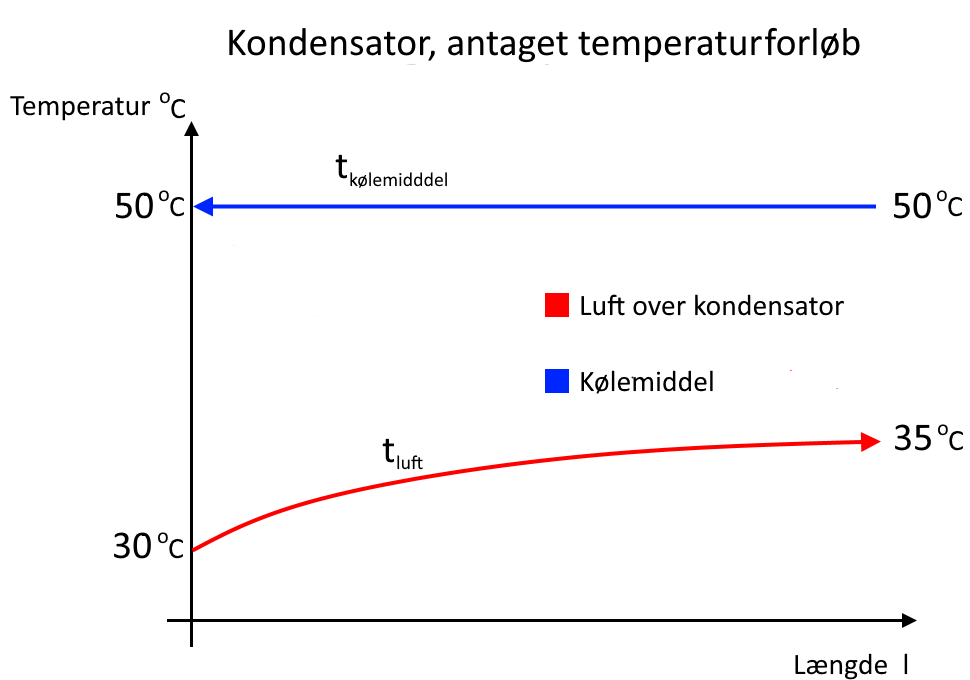
\includegraphics[width=1.00\textwidth]{Billeder/temp_kondens.png} % Venstre billede
	\end{minipage}
	\hfill
	\begin{minipage}[b]{0.485\textwidth}
	\centering
	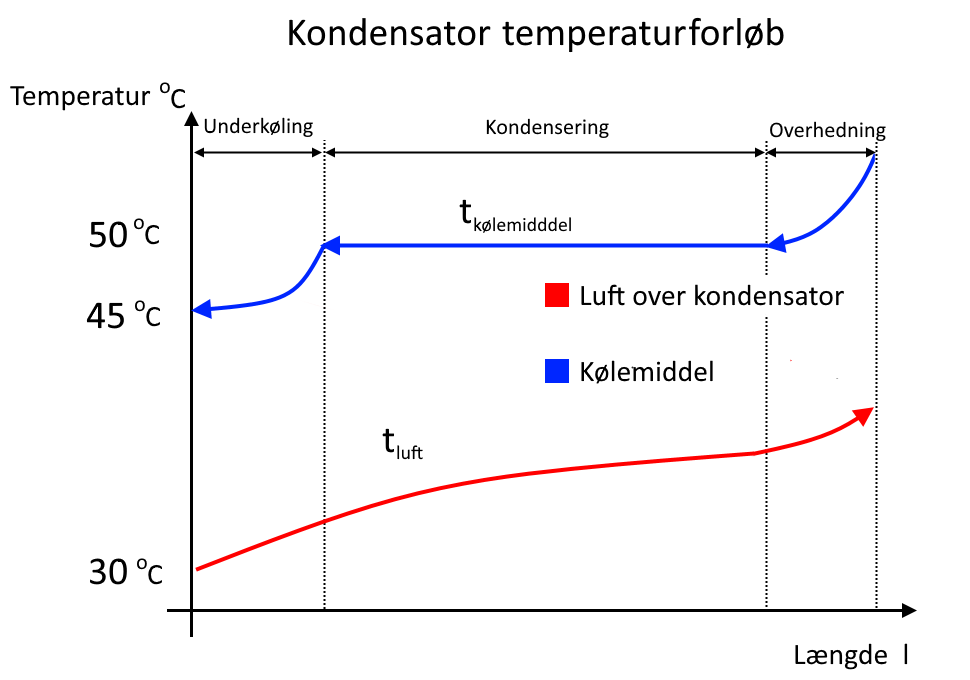
\includegraphics[width=1.00\textwidth]{Billeder/temp_kondens_reel.png} % Højre billede
	\end{minipage}
	\\ % Figurtekster og labels
	\begin{minipage}[t]{0.45\textwidth}
	\caption{\textit{Antaget Temperaturforløb i kondensator}.} % Venstre figurtekst og label
	\label{fig:Konden_tempforloeb_antaget}
	\end{minipage}
	\hfill
	\begin{minipage}[t]{0.45\textwidth}
	\caption{\textit{Reelt temperaturforløb i kondensator}.} % Højre figurtekst og label
	\label{fig:Konden_tempforloeb_reel}
	\end{minipage}
\end{figure}

%-------------------------------   UDVENDIG   ------------------------------------
%---------------------------------------------------------------------------------
%---------------------------------------------------------------------------------
%---------------------------------------------------------------------------------
%---------------------------------------------------------------------------------
%---------------------------------------------------------------------------------


% --- Beregning af den totale varmeovergangsmodstand ---

\subsection{Beregning af den totale varmeovergangsmodstand  (N.J. \& M.N.)}
    \label{sec:Beregning_af_den_totale_varmeovergangsmodstand_kondensator}
For at bestemme kondensatorydelsen, $\si{\Phi_k}$, og  varmegennemgangstallet, U, skal den totale termiske modstand, som varmestrømmen møder fra luften til kølemidlet igennem kondensatorens rør, kendes. Der benyttes samme antagelser for lamel- og rørmaterialer samt for den logaritmiske middeltemperaturdifferens som ved fordamperen i afsnit \ref{sec:Beregning_af_den_totale_varmeovergangsmodstand1}.

\subsection{Beregning af det udvendige varmeovergangstal og overgangsmodstanden, $\alpha_\text{ou}$ og $R_\text{ou}$  (U.H. \& B.B.)}

Det udvendige varmeovergangstal og varmeovergangsmodstanden for varmen fra ribber og rør på kondensatoren til luften bestemmes efter samme beregningsprincipper som i afsnit \ref{sec:Udvendig_varmeovergangsmodstand_fordamper}, hvor det udvendige varmeovergangstal og varmeovergangsmodstanden for fordamperen beregnes. Af tabel \ref{tab:alfa_u_data} fremgår beregningsvariablerne til beregning af det ydre varmeovergangstal og varmeovergangsmodstand:
%--------------------------------------------------------------------------------------
\begin{table}[H] 
\centering
\renewcommand{\arraystretch}{1.2}
\begin{tabular}{|c|c|c|c|}  \rowcolor[gray]{0.7}                                \hline
\multicolumn{4}{|c|}{\textbf{Data til beregning af indre varmeovergangstal}} \\ \hline \rowcolor[gray]{.8}
\textbf{Variabel}   & \textbf{Værdi}        & \textbf{Forklaring} & \textbf{Kilde}    \\ \hline 
c_L & \SI{3}{\frac{m}{s}} & Lufthastighed over kondensatorrør   & Målt \\ \hline 
t_{c}  & \SI{30}{\celsius}     & Lufttemperatur før kondensator    & Antaget \\ \hline 
t_\text{d}  & \SI{35}{\celsius}  & Lufttemperatur efter kondensator  & Gæt \\ \hline 
t_{Lm}  & \SI{32,5}{\celsius}  & Middellufttemperatur ift. $t_{c}$ og $t_{d}$  & Beregnet \\ \hline 
p_{L}  & \SI{1}{\bar}  & Lufttrykket udenfor rørene  & Antaget \\ \hline
\lambda_{L}        & \SI{0.0268}{\frac{W}{m \cdot K}}           & Konduktivitet for luft ved $t_{Lm}$ og $p_{L}$   & EES \\ \hline 
\lambda_{ribbe}        & \SI{237}{\frac{W}{m \cdot K}}           & Konduktivitet for alu. ribber ved $\SI{50}{\celsius}$. & EES \\ \hline 
Pr_{L} & 0,706 & Prandtls Tal for luft ved $t_{Lm}$ og $p_{L}$  & EES \\ \hline 
\nu_{L} & 16,5 \cdot 10^{-6} \si{\frac{m^2}{s}} & Kinematisk viskositet for luft ved $t_{Lm}$ og $p_{L}$ & EES \\ \hline 
m & 0,60 & Konstant, det er geometrisk bestemt af varmeveksler. Tabel \ref{tab:c_og_M} & Tabel \ref{tab:c_og_M} \\ \hline 
C & 0,41 & Konstant, det er geometrisk bestemt af varmeveksler. & Tabel \ref{tab:c_og_M}  \\ \hline 
A_0 & \SI{0,133}{m^2} & Overfladeareal af rør imellem ribber & \ref{eq: Areal af rørstykker mellem ribber}  \\ \hline 
A_t & \SI{1,01}{m^2} & Totalt varmevekslende overfladeareal på kondensator & \ref{eq: Total overfladeareal fordamper}  \\ \hline 
	\end{tabular} 
	\caption{\textit{Variabeloversigt til beregning af den indre varmeovergangstal}} 
	\label{tab:alfa_u_data} 
\end{table} \\

Der beregnes en middelværdi for Nusselts tal udvendigt, som benyttes til at beregne det udvendige varmeovergangstal:
\begin{align}
Re_{L} &= \frac{c_L \cdot d_u}{\nu_L} && = 1460 &&\text{Reynolds tal for luft} \\
Nu_u   &= C \cdot Re_{L}^{m} \cdot \left(\frac{A_t}{A_0} \right) ^{m-1} \cdot Pr_u^{0,33} &&= 12,8 &&\text{Nusselts tal udvendigt - Aages noter} \\
\alpha_\text{ou} &= \frac{Nu_u \cdot \lambda_L}{d_u} &&= \SI{42,9}{\frac{W}{m^2 \cdot K}} &&\text{Udvendig varmeovergangstal} \\
\end{align}
\subsubsection*{Ribbevirkningsgrad}
For at bestemme den udvendige varmeovergangsmodstand, beregnes varmevekslerens ribbevirkningsgrad. Dette foretages på samme vis som i afsnit \ref{sec:Udvendig_varmeovergangsmodstand_fordamper}. Først bestemmes ribbehøjden, $ l_{ribber} $. Heri indgår konstanterne $s_q = \SI{0,025}{m}$ og $s_r = \SI{0,018}{m}$:
\begin{align}
l_{ribber} &= \frac{s_q}{2} - \frac{d_u}{2} &&= 8,50 \cdot 10^{-3}\si{m} &&\text{Ribbehøjden - Danvak ligning 14.7} \\
L          &= l_{ribber} \cdot \sqrt{\frac{2 \cdot \alpha_u}{\lambda_{ribber} \cdot t_{ribber}}} &&= 0,511 &&\text{L, enhedsløs - Danvak ligning 14.7} \\
\beta      &= 1,27 \cdot \sqrt{\frac{\frac{s_r}{2}}{\frac{s_q}{2}}-0,3} &&= 0,823 &&\text{\beta, enhedsløs - Danvak ligning 14.10} \\
\Psi       &= 1+0,35 \cdot \beta \cdot \ln{\left(  \frac{\frac{s_q}{2}}{\frac{d_u}{2}} \right)} &&= 1,33 &&\text{\Psi, enhedsløs - Danvak ligning 14.10}
\end{align}
Hernæst beregnes ribbevirkningsgraden, som benyttes til at beregne den udvendige varmeovergangsmodstand:
\begin{align}
\eta_{ribber} &= \frac{\tanh{(L \cdot \Psi)}}{L \cdot \Psi} &&= 0,870 &&\text{Danvak figur 14.10} \\
R_\text{ou}           &= \frac{1}{\alpha_u \cdot A_t \cdot \eta_{ribber}} &&= \SI{0,0265}{\frac{K}{W}} &&\text{Udvendig termisk modstand}
\end{align}
\subsection{Beregning af varmeledningsmodstanden gennem røret, $R_\text{rør}$ (C.R. \& J.K.)}
Varmeledningsmodstanden igennem røret beregnes efter samme beregningsmæssige principper som i afsnit \ref{sec:VarmeledningsmodstandF} i beregningen for varmeledningsmodstanden i fordamperen. Her slås varmekonduktiviteten for kobber op i \textit{EES} ved \SI{50}{\celsius} til $\lambda_{\text{rør}} = \SI{395}{\frac{W}{m\cdot K}}$. Disse benyttes til at beregne varmeledningsmodstanden:
\begin{align}
R_\text{rør} = \frac{\ln{\frac{d_u}{d_i}}}{2 \cdot \pi \cdot \lambda_{\text{rør}} \cdot L_\text{rør}} = 10,2 \cdot 10^{-6} \si{\frac{K}{W}}
\end{align}

%-------------------------------  INDVENDIG   ------------------------------------
%---------------------------------------------------------------------------------
%---------------------------------------------------------------------------------
%---------------------------------------------------------------------------------
%---------------------------------------------------------------------------------
\subsection{Beregning af indvendig varmeovergangstal og overgangsmodstanden, $\alpha_i$ og $R_i$ (U.H. \& B.B.)}
Kondensatorens indvendige varmeovergangstal vil blive beregnet som ved \citep{koleteknik} afsnit 6.3.3. \\
Den forsimplede beregningsmetode, gældende for Reynolds tal under 35.000, benyttes uanset det endelige Reynolds tal. Dette er nødvendigt, da fremgangsmåden med \textit{Lockhart-Martinelli Parameteren} er yderst kompliceret, hvilket skyldes, at det ved denne metode er nødvendigt at tage adskillige antagelser, som er med til at gøre metoden upræcis. Beregningsformlen fremgår af ligning \ref{eqn:alfa_i}:

%-----------------------------------------------------------------------
\begin{equation}
\label{eqn:alfa_i}
\V{\alpha}_\text{oi}   = 0,555\cdot  \left( \frac {\lambda_{rl}^{3}\cdot \rho_{rl}\cdot  \left( \rho_{rl}-\rho_{rg} \right) \cdot r\cdot g}{\eta_{dyn} \cdot  \left( t_{rk}-t_{v} \right) \cdot d_{i} } \right) ^{0,25}	 
%\mbox{\I \textit{Køleteknik, Ligning 6.39, side 200}}
\end{equation}

Data til beregning af det indvendige varmeovergangstal bestemmes i \textit{EES} og er angivet i tabel \ref{tab:alfa_i_data}:

\begin{table}[H] 
\centering
\renewcommand{\arraystretch}{1.3}
\begin{tabular}{|c|c|c|c|}  \rowcolor[gray]{0.7}                                \hline
\multicolumn{4}{|c|}{\textbf{Data til beregning af indre varmeovergangstal}}                                                   \\ \hline \rowcolor[gray]{.8}
\textbf{Variabel}   & \textbf{Værdi}        & \textbf{Forklaring} & \textbf{Kilde}    \\ 
\lambda_{Rl}        & 70,4 \cdot 10^{-3} \SI{}{\frac{W}{m \cdot K}}           & Konduktivitet for R134a ved $t_{k}$ og $x_L$   & EES \\ \hline

\rho_\text{Rl}   & \SI{1100}{\frac{kg}{m^3}} & Densitet af R134a på væskeform ved $t_{k}$ og $x_L$ & EES \\ \hline 
\rho_\text{Rg}   & \SI{66,3}{\frac{kg}{m^3}} & Densitet af R134a på gasform ved $t_{k}$ og $x_g$ & EES \\ \hline 
r           & \SI{152}{\frac{kJ}{kg}} & Fordampningsentalpi af R134a ved $t_{k}$ & EES \\ \hline 
\eta_\text{dyn} & 142\cdot 10^{-6}\SI{}{\frac{kg}{m\cdot s}} & Dynamisk viskositet for R134a ved $t_{k}$ og $x_L$ & EES \\ \hline 
t_v         & \SI{48}{\celsius}      & Indre vægtemperatur - Antaget til $ t_{k}-\SI{2}{\kelvin}$ hvor: $t_{k}=\SI{50}{\celsius} $                      & Antagelse \\ \hline
% p_\text{oh} & 0,16 & Andel af rørlængden som overheder & Danvak \\ \hline \rowcolor[gray]{.95}
% p_\text{uk} & 0,20 & Andel af rørlængden som underkøles & Danvak \\ \hline \rowcolor[gray]{.95}
	\end{tabular} 
	\caption{\textit{Variabeloversigt til beregning af den indre varmeovergangstal}} 
	\label{tab:alfa_i_data} 
\end{table}
%------------------------------TABEL SLUT-----------------------------
Herefter beregnes det indre varmeovergangstal ved indsætning af data fra tabel \ref{tab:alfa_i_data} i ligning \ref{eqn:alfa_i}:

\begin{equation}
\label{eqn:alfa_i_b}
\V{\alpha}_\text{oi}   = 0,555\cdot  \left( \frac {\lambda_{rl}^{3}\cdot \rho_{rl}\cdot  \left( \rho_{rl}-\rho_{rg} \right) \cdot r\cdot g}{\eta_{dyn} \cdot  \left( t_{k}-t_{v} \right) \cdot d_{i} } \right) ^{0,25} = \SI{2310}{\frac{W}{m^2 \cdot K}}
\end{equation}

Dernæst beregnes den indre termiske modstand. Dette foretages ved beregning af den rørlængde, som går til overhedning og dernæst rørets indre overfladeareal:
\begin{align}
% L_{oh} &= L_\text{rør} \cdot p_{oh}      &&= \SI{0,8448}{m} \tag*{Rørlængde til overhedning}       \\
A_o_i  &= \pi \cdot d_i \cdot L_\text{rør} &&= \SI{0,116}{m^2} &&\text{\text{Indre overfladeareal}} \\
R_\text{oi}    &= \frac{1}{\alpha_i \cdot A_{oi}}  &&= \SI{0,00373}{\frac{K}{W}} &&\text{\text{Indre overgangsmodstand}}                                 
\end{align}
\subsection{Beregning af kondensatorens kapacitet, $\Phi_k$ (J.K. \& C.R.)}
Den samlede termiske modstand benyttes til at bestemme kondensatorens kapacitet. Denne sammenholdes med den kapacitet, som kompressoren kan levere ved det maksimale omdrejningstal.
Den samlede termiske modstand og den logaritmiske middeltemperaturdifferens beregnes:
\begin{align}
    R_{total}= R_\text{oi}+R_\text{rør}+R_\text{oi}= \SI{0,0302}{\frac{K}{W}}
\end{align}
Herefter skal den logaritmiske middeltemperaturdifferens over kondensatoren bestemmes. 
\begin{align}
    \Delta t_m = \frac{\left(t_{k}-t_{c}\right)-\left(t_{k}-t_{d} \right)}{\ln{\left( \frac{t_{k}-t_{c}}{t_{k}-t_{d}} \right)}}= \SI{17,4}{\kelvin}
\end{align}
Som i afsnit \ref{sec:Massestrøm af kølemiddel} er korrektionsfaktoren for krydsstrøm lig med 1. Dermed er den logaritmiske middeltemperaturdifferens givet ved:  
\begin{align}
    \Delta t_{mkryds} = \Delta t_m \cdot \epsilon = \SI{17,4}{\kelvin}
\end{align}
Herefter kan kondensatorydelsen bestemmes til:
\begin{align}
    \Phi_k = \frac{\Delta t_{mkryds}}{R_{sum}} = \SI{576}{\watt}
\end{align}

\subsection{Korrigering for luftens afgangstemperatur (J.K. \& C.R.)}
Ligesom ved beregning på fordamperen (afsnit \ref{sec:dim_fordamper}) er luftens afgangstemperatur gættet. Denne spiller en rolle i udregning af kondensatorydelsen. Derfor vil afgangstemperaturen i dette afsnit blive præciseret gennem en iterativ proces. Luftens afgangstemperatur beregnes ud fra samme fremgangsmåde som beskrevet i afsnit \ref{sec:afgangstemp_fordamp}.
Ud fra den bestemte kondensatorydelse, vil luftens afgangstemperatur blive beregnet ud fra energibalancen for luft over kondensatoren:
\begin{equation}
    q_\text{mL}\cdot (h_\text{c} - h_\text{d}) + \Phi_k = 0
\end{equation}
Bestemte værdier samt resultater heraf fremgår af nedenstående tabel:
\begin{table}[H]
\centering
\begin{tabular}{|c|c|}
\hline
\rowcolor[HTML]{C0C0C0} 
\multicolumn{2}{|c|}{\cellcolor[HTML]{C0C0C0}\textbf{Resultat af iterativ proces}} \\ \hline
\rowcolor[HTML]{EFEFEF} 
\textbf{Betegnelse}     & \textbf{Værdi}            \\ \hline
$\rho_\text{Lm}$        & \SI{1,14}{\frac{kg}{m^3}} \\ \hline
$A_\text{L}$            & \SI{0,0278}{m^2}          \\ \hline
$q_\text{mL}$           & \SI{0,0951}{\frac{kg}{s}} \\ \hline
$h_\text{d}$            & \SI{309}{\frac{kJ}{kg}}   \\ \hline
$t_\text{d,beregnet}$   & \SI{36,0}{\celsius}       \\ \hline
\end{tabular}
\caption{\textit{Resultatet af beregningerne til kondensatoren}.}
\label{tab:kond_it_1}
\end{table}

Derefter vil samtlige udregninger, til beregning af kondensatorens ydelse, blive udført med en ny værdi for luftens afgangstemperatur, $t_\text{d}$. Dette gøres indtil værdien for denne og $t_\text{d,beregnet}$ er sammenfaldende.
Efter endt iterativ proces er resultaterne af kondensatorens ydelse fundet til nedenstående:

\begin{table}[H]
\centering
\begin{tabular}{|c|c|}
\hline
\multicolumn{2}{|c|}{\cellcolor[HTML]{C0C0C0}\textbf{Resultat efter iterativ proces}} \\ \hline
$t_\text{d}$   & \SI{35,9}{\celsius}   \\ \hline
$\Phi_k$        & \SI{559}{W} \\ \hline
$U_\text{u}$    & \SI{32.7}{\frac{W}{m^2 \cdot K}} \\ \hline
\end{tabular}
\caption{\textit{Resultatet er beregningerne til kondensatorens ydelse}.}
\label{tab:kond_it_2}
\end{table}


\subsection{Delkonklusion (Alle)}
Det fremgår ud fra ovenstående beregninger at kondensatorkapaciteten på \SI{559}{\watt} ved de givne driftsforhold er opfyldt. Dette gælder både for den oplyste værdi i \citep{Coolselector} på \SI{530}{\watt} og den værdi, som er blevet udregnet i afsnit \ref{sec:kondenseringsydelse_med_koling} på \SI{483,9}{\watt}. Eftersom kondensatorens kapacitet overstiger disse værdier, vil kondenseringstryk- og temperatur reduceres, hvilket resulterer i en højere effektfaktor.  
Desuden er luftens udgangstemperatur fundet ved de givne driftsforhold, gennem en iterativ proces, til \SI{35,9}{\celsius}.  
\end{document}
